\section{模型检验、敏感性与稳健性分析}

\subsection{物理可行性与因果性检验}

对问题一及四个年度主策略逐槽检查式\eqref{eq:balance}、式\eqref{eq:soc}、SOC边界、充放电功率、非负性、同时充放和跨日连续性。问题一最大母线平衡残差为 $9.10\times10^{-13}\,\mathrm{kWh}$；四个主策略正式统计期的最大平衡残差不超过 $3.70\times10^{-13}\,\mathrm{kWh}$，独立逐槽重算的最大SOC递推残差约为 $4.55\times10^{-12}\,\mathrm{kWh}$。这些量接近浮点运算精度，表明结果满足模型物理方程。

因果性检验在第0、1和364日的0、2、\ldots、22时，对未来负荷、光伏、价格和未发布预报分别作36组扰动。当前预测、价格估计和当前LP计划的最大差均为0；已执行前缀和SOC边界也不受未来扰动影响。这验证了实现遵守信息集 $\mathcal F_{d,h}$。该检验说明“没有使用被扰动的未来数据”，但不是对所有可能代码路径的形式化证明。

\subsection{54组实验设计}

实验共54组，其中16组为固定价/变价的安全轨迹、点预测、典型日、无储能，以及0/12/6/2小时更新基线；另有38组单因素实验。单因素范围包括：
\begin{itemize}
  \item 保守分位参数 $\alpha=0.70,0.75,0.80,0.85,0.90,0.95$；
  \item 残差聚类上限5、9、12、16，残差历史30、60、90日；
  \item 储能容量和功率分别为主值的0.8、1.0、1.2倍；
  \item 往返效率从0.81提高到0.90，即单向效率改为 $\sqrt{0.9}$；
  \item 应急电价倍率3、4、5、6、8。
\end{itemize}
容量改变时，SOC下限、上限和初态仍分别为容量的10\%、90\%和50\%，而功率与效率保持不变；功率实验则不改变容量。应急倍率实验固定物理策略和 $\alpha=0.8$，只重新计算费用暴露，因此不能称为各倍率下重新寻优的最优策略。

\subsection{保守参数与设备参数}

图\ref{fig:q4-alpha}展示 $\alpha$ 对费用和应急量的权衡。固定价问题二中，$\alpha=0.95$ 的样本内费用低于主设定0.8；变价有调账方案中，0.8是测试点中的最低费用。由于主参数在查看本年度结果前固定，本文不据此把0.95或0.8宣称为普适最优参数。样本内曲线的主要价值在于说明保守度改变会同时影响合同过购、应急缺口和弃光，而不是提供无偏超参数选择。

\begin{figure}[H]
  \centering
  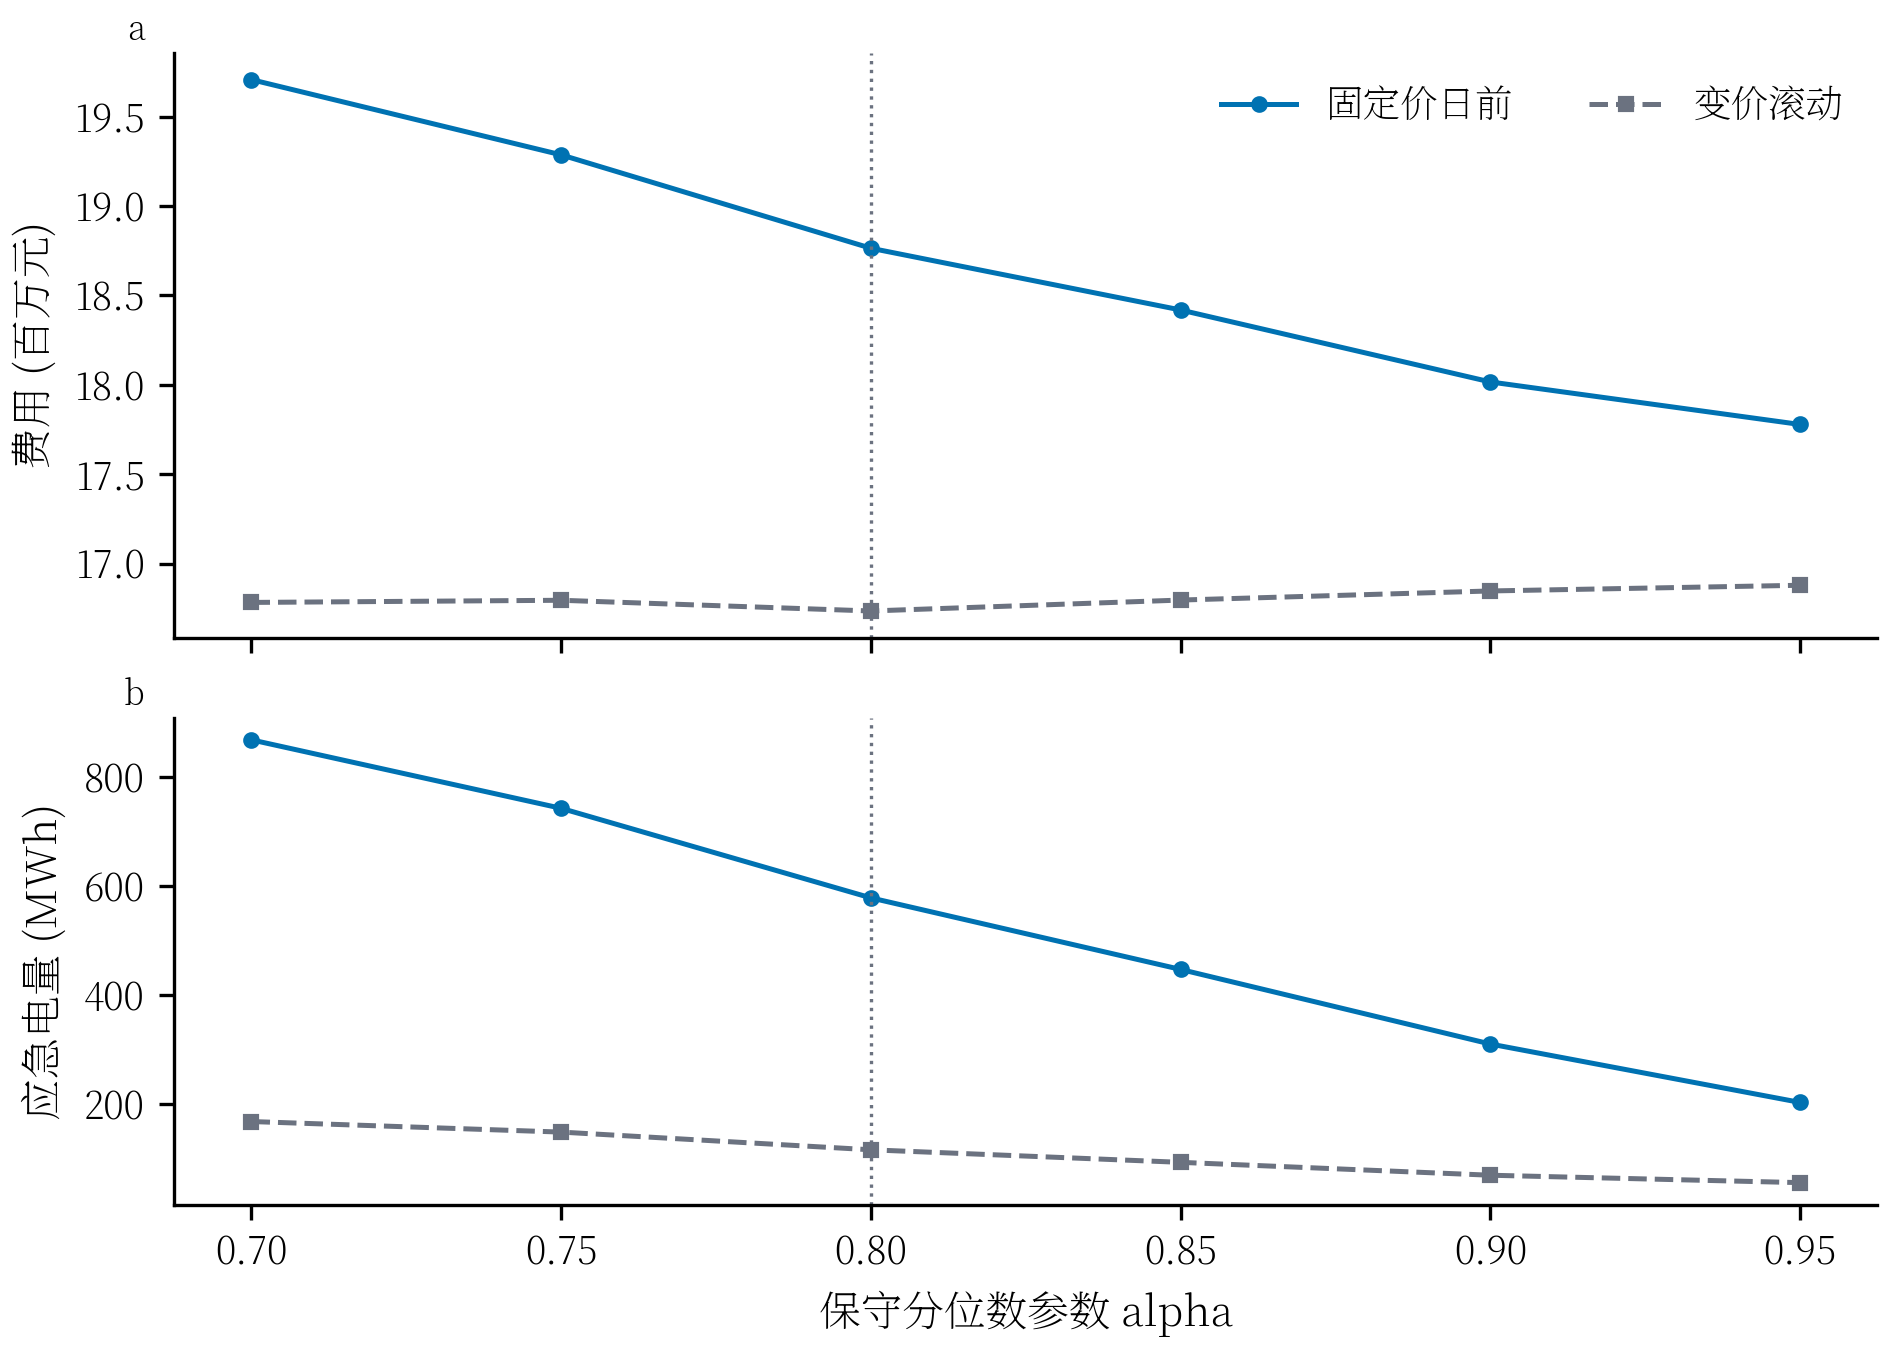
\includegraphics[width=0.96\textwidth]{figs/result_q4_alpha_sensitivity.png}
  \caption{问题二与问题四有调账策略对保守分位参数的单因素敏感性。主方案 $\alpha=0.8$ 为事前固定值。}
  \label{fig:q4-alpha}
\end{figure}

历史窗口30日时，问题二和问题四有调账方案费用分别约为1698.74万元和1629.52万元；90日窗口更高。这反映2025年样本中的近期结构更有用，但不证明短历史在其他年份总是更好。容量增加20\%后，两方案费用分别约为1821.87万元和1600.59万元；容量减少20\%并不必然按比例增加费用，因为合同风险、弃光和终端SOC共同变化。

表\ref{tab:sensitivity-selected}列出若干有代表性的单因素结果。历史窗口30日对两个方案都较有利，说明2025年数据存在较强的近期性；提高往返效率则稳定降低费用。容量增加对问题四有调账方案的收益大于对问题二，原因是变价环境下额外可用能量同时具有峰谷转移和风险缓冲价值。所有比较都只改变表中一个因素，其余参数保持主设定。

\begin{table}[H]
\centering
\caption{部分单因素实验的334日现金费用（万元）}
\label{tab:sensitivity-selected}
\begin{tabular}{lrr}
\toprule
实验设置 & 问题二无调账 & 问题四有调账\\
\midrule
主设定 & 1876.42 & 1673.51\\
残差历史30日 & 1698.74 & 1629.52\\
储能容量增加20\% & 1821.87 & 1600.59\\
储能功率降至80\% & -- & 1669.53\\
往返效率提高到90\% & 1832.77 & 1620.57\\
\bottomrule
\end{tabular}
\end{table}

问题四有调账方案将功率降至主值的80\%时，样本内费用约为1669.53万元，略低于主方案1673.51万元。这一非单调性并不违反物理规律：控制器采用保守轨迹规划和真实值下的贪心执行，并非在完全信息下对全年重新全局优化；更大的设备可行域不会自动保证启发式滚动策略产生更低的实际结算费用。往返效率提高到90\%后，费用下降到约1620.57万元，符合损耗降低的方向性预期。

实验还揭示了初态与年末状态的关系。所有容量实验都从容量的50\%起步，SOC上下界同步保持10\%和90\%；这保证比较不是由绝对初态不一致造成。然而，正式费用从2月开始统计，1月调度已经把不同容量系统推进到各自状态，因此不能简单断言初始SOC影响在一个月后完全消失。本文只报告统一启动规则下的可比结果，不对无限期稳态作额外假设。

\subsection{结算与时间口径敏感性}

同一策略在主结算和替代结算下费用差异明显。问题三主策略由1627.97万元增至1707.60万元，问题四有调账策略由1673.51万元增至1749.07万元。更重要的是，2小时相对6小时的收益在替代口径下明显收缩。因此，更新频率结论必须与式\eqref{eq:settlement-primary}绑定，不能只给一个脱离合同条款的百分比。

固定价方案还出现排序反转：主结算下12小时方案费用低于仅0时方案，而替代重计费下仅0时方案约1761.33万元，反而低于12小时方案约1773.52万元。其原因不是物理供能突然变化，而是替代规则对合同下调额外收费。该现象说明，调账价值必须同时报告物理效果和条款效果；仅凭“应急减少”不足以得出经济最优结论。

时间口径实验把典型日全部槽循环平移10分钟。购电总量仅有约 $2.38\times10^{-9}\,\mathrm{kWh}$ 的浮点差，而费用下降约0.10元。结果表明年度策略量级不依赖这一微小映射，但题目指定时段数值和逐槽费用仍需要统一定义，本文采用区间终点解释。

\subsection{计算规模与结果可追溯性}

每天的规划域最多为144槽，随着日内时间推进逐步缩短。每槽包含合同、闲置合同、光伏利用、充电、放电、应急与SOC等连续变量，约束数量随剩余槽数线性增长；所有目标和约束均为线性形式，可由通用线性规划器稳定求解。残差聚类的数据矩阵最多含60个历史日期、每行288维，且簇数不超过9，因此其规模远小于把全年每个10分钟误差都展开成场景树的做法。该结构使365日连续模拟和54组实验在普通计算机上可完成，同时保留逐槽检查的可能。

为了使结果可追溯，每个策略同时保留三层输出：第一层是逐槽合同、能量流和SOC，用于检查式\eqref{eq:balance}、式\eqref{eq:soc}及指定时段；第二层是每日合同量、现金费用、应急量、闲置合同和弃光，用于代表日与时间序列分析；第三层是334日总量及实验参数，用于跨策略比较。论文中的所有汇总均从前一层按日期和时槽聚合，而不是在正文中手工修改。题目指定的五份工作簿与同一逐槽结果共用数据源，所以论文数值、代表日表和Excel输出保持同一口径。

随机性只出现在残差聚类的初始中心，随机种子固定为2026，并使用10次初始化选择较小簇内平方和的结果。经验分位数、相似日权重、价格中位数、LP和真实执行均为确定性步骤。固定种子并不说明模型没有统计不确定性，它只确保相同输入和软件环境下不会因聚类初始化改变合同轨迹。真正的外部不确定性仍来自未来负荷、光伏和价格，已通过滚动历史、分位参数与应急购电显式暴露。

结果解释遵循“数值可行、因果可用、外部有效性待检验”的层次。逐槽残差接近机器精度证明计算结果满足本文方程；未来扰动不影响当前决策证明实现遵守给定信息边界；54组实验说明主要参数变化下结论如何移动。但这些证据不能自动证明另一年份、另一微网或另一合同条款下仍有同样节约率。工程迁移时应先复现输入映射和结算，再用滚动样本外数据重新校准历史窗口与保守度。

\subsection{模型优点与局限}

本文方法具有四点优点：第一，信息集明确，预测与执行均可通过未来扰动验证；第二，物理层完全线性，所有10分钟结果可逐槽复核；第三，联合残差在压缩前同时包含负荷和光伏误差，较单独安全系数更贴近净负荷风险；第四，两种结算、多个更新集合和设备参数均有真实重算或同策略重计费结果。

局限也十分明确。其一，边际分位压缩会丢失跨时段联合概率，不能提供机会约束保证。其二，相似日和历史中位数属于低参数预测，可能无法捕捉节假日、极端天气或结构突变。其三，真实执行采用优先级规则而非全年完美信息优化，设备参数的实际费用可能非单调。其四，储能老化、备用、配网潮流和需求响应不在题设数据中，本文没有虚构这些成本；若用于工程实施，应加入退化成本、网络约束和滚动终端集合。其五，2小时方案是由已发布预报与观测构成的合成短临结果，不能替代对真实高频预报服务的独立评估。
